\documentclass[12pt,leqno]{article}
\usepackage{amssymb}
\usepackage{amsrefs}
\usepackage{verbatim}
\usepackage{array}

%\usepackage{showlabels}
%\usepackage{pifont}
\usepackage{tikz}
\newcommand*\circled[1]{\tikz[baseline=(char.base)]{
            \node[shape=circle,draw,inner sep=2pt] (char) {#1};}}
\usepackage{rotating}
\usepackage{amsmath}
\usepackage{tabularx}
\usepackage{caption}
\usepackage{theorem}
\usepackage[matrix,tips,frame,color,line,poly]{xy}
%\usepackage[dvips]{graphicx}

\renewcommand{\labelenumi}{(\arabic{enumi})}

\newtheorem{theorem}[equation]{Theorem}
\newtheorem{corollary}[equation]{Corollary}
\newtheorem{definition}[equation]{Definition}
\newtheorem{lemma}[equation]{Lemma}
\newtheorem{desideratum}[equation]{Desideratum}
\newtheorem{conjecture}[equation]{Conjecture}
\newtheorem{proposition}[equation]{Proposition}
\newtheorem{remark}[equation]{Remark}
{\theorembodyfont{\rmfamily}
\newtheorem{theoremplain}[equation]{Theorem}
\newtheorem{remarkplain}[equation]{Remark}
\newtheorem{editorialremarkplain}[equation]{Editorial Remark}
\newtheorem{exampleplain}[equation]{Example}
\newtheorem{corollaryplain}[equation]{Corollary}
}
\newcommand{\qed}{\hfill $\square$ \medskip}
\newenvironment{proof}[1][Proof]{\noindent\textbf{#1.} }{\qed}
\newcommand\exact[3]{1\rightarrow #1\rightarrow #2\rightarrow #3\rightarrow1}
\newcommand{\Aut}{\text{Aut}}
\newcommand{\sgn}{\text{sgn}}
\newcommand{\sig}{\text{sig}}
\newcommand{\hodge}{\text{hodge}}
\newcommand{\triv}{\text{triv}}
\newcommand{\diag}{\text{diag}}
\newcommand{\codim}{\text{codim}}
\newcommand{\gr}{\text{gr}}
\newcommand{\Out}{\text{Out}}
\newcommand{\Int}{\text{Int}}
\renewcommand{\int}{\text{int}}
\newcommand{\h}{\mathcal H}
\renewcommand{\j}{\mathcal J}
\newcommand{\Hreg}{H_{\text{reg}}}
\newcommand{\reg}{\text{reg}}
\newcommand{\Hom}{\text{Hom}}
\newcommand{\mult}{\text{mult}}
\newcommand{\Ind}{\text{Ind}}
\newcommand{\End}{\text{End}}
\newcommand{\PS}{\text{PS}}
\newcommand{\ad}{\text{ad}}
\newcommand{\Ad}{\text{Ad}}
\newcommand{\Lie}{\text{Lie}}
\newcommand{\Stab}{\text{Stab}}
\newcommand{\Norm}{\text{Norm}}
\newcommand{\Cent}{\text{Cent}}
\newcommand{\X}{\mathcal X}
\newcommand{\Y}{\mathcal Y}
\newcommand{\caZ}{\mathcal Z}
\newcommand{\caM}{\mathcal M}
\newcommand{\caI}{\mathcal I}
\newcommand{\I}{\mathcal I}
\renewcommand{\O}{\mathcal O}
\renewcommand{\S}{\mathcal S}
\newcommand{\caN}{\mathcal N}
\newcommand{\caW}{\mathcal W}
\newcommand{\caP}{\mathcal P}
\newcommand{\caH}{\mathcal H}
\newcommand{\caPreg}{\mathcal P_{\text{reg}}}
\newcommand{\chPreg}{\ch P_{\text{reg}}}
\newcommand{\caT}{\mathcal T}
\newcommand{\caC}{\mathcal C}
\newcommand{\caA}{\mathcal A}
\newcommand{\tX}{\widetilde{\mathcal X}}
\newcommand{\tS}{\widetilde{\mathcal S}}
\newcommand{\tL}{\widetilde{\mathcal L}}
\newcommand{\tP}{\widetilde{\mathcal P}}
\newcommand{\tx}{\widetilde{x}}
\newcommand{\tphi}{\widetilde{\phi}}
\newcommand{\F}{\mathbb F}
\newcommand{\R}{\mathbb R}
\newcommand{\C}{\mathbb C}
\newcommand{\Z}{\mathbb Z}
\newcommand{\W}{\mathbb W}
\newcommand{\Ztwo}{\mathbb Z/2\Z}
\newcommand{\N}{\mathbb N}
\newcommand{\Q}{\mathbb Q}
\renewcommand{\F}{\mathbb F}
\newcommand{\E}{\mathcal E}
\newcommand{\caD}{\mathcal D}
\newcommand{\caS}{\mathcal S}
\newcommand{\caL}{\mathcal L}
\newcommand{\caB}{\mathcal B}
\newcommand{\chcaD}{\mathcal D^\vee}
\newcommand{\T}{\mathbb T}
\newcommand{\G}{G}
\renewcommand{\H}{\mathbb H}
{\renewcommand{\h}{\mathfrak h}}
\renewcommand{\q}{\mathfrak q}
\renewcommand{\u}{\mathfrak u}
\renewcommand{\a}{\mathfrak a}
\newcommand{\A}{\mathbb A}
\newcommand{\K}{\mathbb K}
\newcommand{\B}{\mathbb B}
\newcommand{\spint}{\widetilde{Spin}}
\newcommand{\tH}{\widetilde H}
\newcommand{\tG}{\widetilde G}
\newcommand{\tW}{\widetilde W}
\newcommand{\tK}{\widetilde K}
\newcommand{\tD}{\widetilde D}
\newcommand{\bD}{\overline D}
\newcommand{\bp}{\overline\Pi}
\newcommand{\tM}{\widetilde M}
\newcommand{\dual}[2]{^{#1}#2}
%\newcommand{\Ch}[1]{#1{\text{\large\v{}}}}
\newcommand{\ch}[1]{#1^\vee}
%\newcommand{\ch}[1]{{\text{\large\v{}}}#1}
\newcommand{\chG}{\ch{G}}
\newcommand{\chT}{\ch{T}}
\newcommand{\tildeint}{{\~{}\it{--integral}}\ }
\renewcommand{\L}[1]{^L#1}
\renewcommand{\sec}[1]{\section{#1}
\renewcommand{\theequation}{\thesection.\arabic{equation}}
  \setcounter{equation}{0}}
\newcommand{\subsec}[1]{\subsection{#1}
\renewcommand{\theequation}{\thesubsection.\arabic{equation}}}
\renewcommand{\t}{\mathfrak t}
\newcommand{\mi}{\medskip\noindent}
\newcommand{\si}{\smallskip\noindent}
\newcommand{\g}{\mathfrak g}
\newcommand{\GGamma}{G^\Gamma}
\newcommand{\GGammaG}{G^\Gamma\backslash G}
\newcommand{\chGGamma}{G^{\vee\Gamma}}
\newcommand{\WGamma}{W^\Gamma}
\newcommand{\weil}{W_\R}
\newcommand\inv{^{-1}}
\newcommand\bs{\backslash}
\newcommand\wt{\widetilde}
\newcommand\fix[1]{{\noindent\bf#1}}
\newcommand\kgb{{\tt KGB}}
\newcommand{\Khat}{\widehat K}
\newcommand{\Wconj}{[W]}
\newcommand{\Weconj}{[{W_e}]}
\newcommand{\Gssconj}{[{G^\text{ss}}]}
\newcommand{\Gss}{G^\text{ss}}
\newcommand{\Wext}{\negthinspace\negthinspace\phantom{a}^\delta W}
\newcommand{\Text}{\negthinspace\negthinspace\phantom{a}^\delta T      }

\def\fh{\mathfrak h}
\def\fg{\mathfrak g}
\def\fc{\mathfrak c}
\def\fm{\mathfrak m}
\def\ft{\mathfrak t}
\def\fs{\mathfrak s}
\def\fb{\mathfrak b}
\def\fp{\mathfrak p}
\def\fl{\mathfrak l}
\def\fn{\mathfrak N}
\def\fA{\mathfrak A}
\def\fH{\mathfrak H}
\def\fP{\mathfrak P}
\def\fU{\mathfrak U}
\def\fu{\mathfrak u}
\def\fo{\mathfrak o}
\def\fS{\mathfrak S}

\def\ge{\geqslant}
\def\le{\leqslant}
\def\a{\alpha}
\def\b{\beta}
\def\g{\gamma}
\def\G{\Gamma}
\def\d{\delta}
\def\D{\Delta}
\def\L{\Lambda}
\def\e{\epsilon}
\def\et{\eta}
\def\io{\iota}
\def\o{\omega}
\def\p{\pi}
\def\ph{\phi}
\def\ps{\psi}
%\def\r{\rho}
\def\s{\sigma}
\def\t{\tau}
\def\th{\theta}
\def\k{\kappa}
\def\l{\lambda}
\def\z{\zeta}
\def\v{\vartheta}
\def\x{\xi}
\def\i{^{-1}}

\renewcommand{\sec}[1]{\section{#1}
\renewcommand{\theequation}{\thesection.\arabic{equation}}
  \setcounter{equation}{0}}
\font\temporary=manfnt
\def\dbend{{\temporary\char127}} % dangerous bend sign
% Danger, Will Robinson!
\def\danger{\begin{trivlist}\item[]\noindent%
\begingroup\hangindent=3pc\hangafter=-2%\clubpenalty=10000%
\def\par{\endgraf\endgroup}%
\hbox to0pt{\hskip-\hangindent\dbend\hfill}\ignorespaces}
\def\enddanger{\par\end{trivlist}}

\begin{document}
\title{From the Weyl group to conjugacy classes of finite order}
\author{Jeffrey Adams, Xuhua He and Sian Nie}
\maketitle

\sec{Introduction}

Let $G$ be a connected reductive group over $\C$.
Choose a Cartan subgroup $T\subset G$, let $N(T)$ be the normalizer of $T$ in $G$,
and let $W=N(T)/T$ be the Weyl group.
We have the exact sequence
\begin{equation}
\label{e:exactW}
1\rightarrow T\rightarrow N(T)\overset p\rightarrow W\rightarrow 1.
\end{equation}
In \cite{AH} we considered the question of whether this sequence splits,
and more generally if $w\in W$, what can be said about the order of $p\inv(w)$.
Here we consider a related problem.

Let $\Wconj$ be the set of conjugacy classes in $W$. Let $\Gss$ be the
semisimple elements of $G$, and $\Gssconj$ the set of semisimple
conjugacy classes. We have $N(T)\subset \Gss$. For $w\in W$ write $[w]$ for the the $W$-conjugacy
class of $w\in W$. Similarly for $g\in \Gss$ let $[g]$ be
$G$-conjugacy class of $g$.

Suppose $w\in W$ and $n_w\in p\inv(w)\in N(T)$. For general $w$ there
are many choices of $n_w$, even up to conjugacy. For example if $w=1$
then $n_w$ is any element of $T$. In an important special case the
choice of $n_w$ is unique up to conjugation. We say $w\in W$ is elliptic
if it has no nontrivial fixed vectors in the reflection
representation.


\begin{lemma}
Suppose $w\in W$ is elliptic. Then any two elements of
$p\inv(w)\subset N(T)$ are $T$-conjugate. Therefore the map $w\rightarrow n_w\in p\inv(w)$ induces
a well-defined map
$$
\Psi:[w]\rightarrow [t_w]: \Weconj\rightarrow\Gssconj.
$$
\end{lemma}
This map has been studied by many people \dots on a case-by-case
basis. Our main result is a uniform algorithm to compute this map. We
also consider the twisted case where $W$ is replaced by $\Wext$, the
semidirect product of $W$ and a distinguished involution of finite
order.

\sec{The Algorithm}\label{const}

Let $G,T,N(T),W$ be as in the introduction.  We say an automorphism of
$G$ is {\it distinguished} if it preserves some splitting datum
$(G,T,\{X_\alpha\})$. Recall an inner automorphism is distinguished if
and only if it is trivial, and the outer automorphism group of $G$ is
isomorphic to the group of automorphisms of a splitting datum. See ?.

Now suppose $\delta$ is a distinguished automorphism of $G$ of finite
order, preserving a splitting datum $(G,T,\{X_\alpha\})$. Then
$\delta$ induces an automorphism, also denoted $\delta$ of $W$, and we define
$$
{}^\d G=G \rtimes\langle\delta\rangle, \quad \Wext=W\rtimes\langle\delta\rangle.
$$


Let $\Delta=\Delta(T,G)$ be the root system, and
$V=\R\langle\Delta\rangle$. This is a representation of $\Wext$ which
we refer to as the reflection representation.


We fix a set $\Delta^+\subset\Delta$ of positive roots.
Let $\Pi$ be the corresponding set of simple roots, and $\caC$ be the corresponding dominant chamber,

Suppose $w\in \Wext$. Let
\begin{subequations}
\renewcommand{\theequation}{\theparentequation)(\alph{equation}}
\label{e:algorithm}
\begin{equation}
\Gamma_w=\{0\le\theta\le\pi\mid\text{such that } e^{i\theta}\text{ is an eigenvalue of $w$\text{ on }V\}}
\end{equation}
Write
\begin{equation}
\label{e:thetas}
\Gamma_w=\{\theta_1,\theta_2,\dots,\theta_k\}\text{ with }\theta_1<\theta_2<\dots<\theta_k.
\end{equation}
For $\theta\in \Gamma_w$ let
\begin{equation}
V(w,\theta)=\{v\in V\mid w(v)+w\inv(v)=2\cos(\theta)v\}.
\end{equation}
Then $V(w,\theta)\otimes_\R\C$ is the direct sum of the eigenspaces of
$w$ on $V\otimes_\R\C$ with eigenvalue $e^{\pm i\theta}$.

Set
$$
F_i=\sum_{j=1}^i V(w,\theta_j)\quad(\le i\le k)
$$
and set $F_0=0$ so we have a filtration
\begin{equation}
0=F_0\subsetneqq F_1\dots \subsetneqq \dots\subsetneqq F_{k}=V
\end{equation}
with strict containments. Set
\begin{equation}
\Delta_i=\{\alpha\in\Delta\mid \langle\alpha,F_i\rangle=0 \quad(0\le i\le k)
\end{equation}
Then each $\Delta_i$ is a root system, and set
\begin{equation}
W_i=W(\Delta_i).
\end{equation}
Thus we have
\begin{equation}
\begin{aligned}
\Delta&=\Delta_0\supseteq \Delta_1\supseteq \dots\supseteq \Delta_k=\emptyset\\
W&=W_0\supseteq W_1\supseteq \dots\supseteq W_k=\{1\}\\
\end{aligned}
\end{equation}
For each $i$ set
\begin{equation}
\begin{aligned}
\Delta^+_i&=\Delta^+\cap \Delta_i\\
\ch\rho_i&=\frac12\sum_{\alpha\in\Delta_i^+}\ch\alpha
\end{aligned}
\end{equation}
We define rational coweights
$\{\ch\lambda_0,\dots, \ch\lambda_{k}\}$ by downward induction.
Set $\ch\lambda_k=0$, and for $0\le i\le k-1$ define
\begin{equation}
\begin{aligned}
\ch\lambda_{i}=\frac{d(\theta_{i+1}-\theta_{i})}{2\pi}\ch\rho_i+\overline{\ch\lambda_{i+1}}
\end{aligned}
\end{equation}
where $\overline{\ch\lambda_{i+1}}$ is the element in the $W_i$-orbit of $\ch\lambda_{i+1}$ which is dominant for $\Delta^+_i$.
\end{subequations}

\begin{theorem}
\label{t:main}
Suppose $w\in W\delta\subset \Wext$ is elliptic. Construct $\ch\lambda_0$ by the algorithm. Then
$$
\Psi([w])=[\delta e^{\frac{2\pi i\ch\lambda_0}d}].
$$
\end{theorem}
\begin{remark}
The algorithm here uses the full sequence $(\th_1, \ldots,
\th_k)$.
One may replace the full sequence by any subsequence that is
admissible in the sense of \cite[subsection 5.2]{he_nie_minimal_finite}. The element
$\delta e^{\frac{2\pi i\ch\lambda_0}d} \in {}^\d G$ obtained from an
admissible subsequence of $(\th_1, \ldots, \th_k)$ is, in general,
different from the element obtained here using the full
sequence. However, these elements are all conjugate to $n_w$. See
example \ref{eg:regular}.
\end{remark}

{\bf To Jeff, the map $\Psi$ is only defined for nontwisted case in the introduction}

\sec{Digression on the good elements}

\subsection{} The algorithm we gave above is partially motivated by
the construction of the good elements in a given conjugacy class of
$\Wext$. In this section, we make a digression and discuss this
construction.

The good elements in $W$ are introduced by Geck and Michel in
\cite{geck_michel_good} and the notion is generalized to $\Wext$ by Geck, Kim and
Pfeiffer in \cite{gkp}.

Let $B^+$ be the braid monoid associated with $(W,S)$. Then there is a
canonical injection $j:W\longrightarrow B^+$ identifying the
generators of $W$ with the generators of $B^+$ and
$j(w_1w_2)=j(w_1)j(w_2)$ for $w_1,w_2\in W$ such that
$\ell(w_1w_2)=\ell(w_1)+\ell(w_2)$.

Now the automorphism $\delta$ induces an automorphism of $B^+$, which
is still denoted by $\delta$. Set ${}^{\delta} B^+=B^+ \rtimes
\langle\delta\rangle$. Then $j$ extends in a canonical way to an
injection $\Wext \to {}^{\delta} B^+$, which we still denote by
$j$. We will simply write $\underline w$ for $j(w)$.

By definition, $w \in \Wext$ is a {\it good element} if there exists a
strictly decreasing sequence $\Pi_0 \supsetneq \Pi_1 \supsetneq \cdots
\supsetneq \Pi_l$ of subsets of $\Pi$ and even positive integers
$d_0,\cdots,d_l$ such
that $${\underline{w}}^d=\underline{w_0}^{d_0}\cdots\underline{w_l}^{d_l}.$$
Here $d$ is the order of $w$ and $w_i$ is the longest element of the
parabolic subgroup of $W$ generated by $\Pi_i$.

It was proved in \cite{geck_michel_good}, \cite{gkp} and \cite{he_minimal_length_double_cosets} that for any
conjugacy class of $\underline W$, there exists a good minimal length
element. In \cite{he_nie_minimal_finite}, the second and third-named authors  
(wrong reference: only 2 authors?) give a
general proof, which also provides an explicit construction of good
minimal length elements.

Now we recall the construction in \cite{he_nie_minimal_finite}.

Let $\caA$ be a Weyl chamber and for $0 \le i < k$, let $\caC_i(\caA)$
be the connected component of $V-\cup_{H_\a; F_i \subset H_\a}H$
containing $\caA$. We say $\caA$ is in {\it good position} with
respect to $w$ if for any $i$, the closure $\overline{\caC_i(\caA)}$
contains some regular point of $F_{i+1}$.

By \cite[Lemma 5.1]{he_nie_minimal_finite}, there exists some Weyl chamber $\caA$ that is
in good position with respect to any given $w$. By definition, for any
$x \in W$, the Weyl chamber $x(\caA)$ is in good position with respect
to $x w x^{-1}$. In particular, for any conjugacy class of $\Wext$,
there exists an element $w$ such that the dominant chamber is in good
position with respect to $w$. In this case, $\D_i$ is the root system
of the standard Levi subgroup of $G$ associated to the subset
$\Pi_i:=\Pi \cap \D_i$ of simple roots and $W_i=W_{F_i}$ is a standard
parabolic subgroup of $W$ for any $i$. We denote by $W^{\Pi_i}$ the
set of minimal length representatives in $W/W_i$. By \cite[Proposition
2.2]{he_nie_minimal_finite}, we have the following good factorization of $w$.

\begin{proposition}\label{good-fac} Let $w \in W \d \subset
\Wext$. Suppose that the dominant chamber is in good position with
respect to $w$. Then $$w=\d x_1 x_2 \cdots x_k,$$ where for $1 \le i
\le k$, we have $x_i \in W_{i-1} \cap W^{\Pi_i}$ and $\d_i=\d x_1
\cdots x_{i}$ such that $\d_i (\Pi_i)=\Pi_i$.
\end{proposition}

The following result is proved in \cite[Theorem 5.3]{he_nie_minimal_finite}.

\begin{theorem} Let $w \in \Wext$ such that the fundamental chamber is
in good position with $w$. Then we have the following equality in the
Braid monoid associated with $(W, S)$: $$\underline w^d=\underline
w_0^{d \theta_1/\pi} \underline w_1^{d (\theta_2-\theta_1)/\pi} \cdots
\underline w_{k-1}^{d (\theta_{k}-\theta_{k-1})/\pi},$$ where $d$ is
the order of $w$ in $\Wext$, $\underline \theta_0=(\theta_1, \cdots,
\theta_k)$ is the sequence consisting of all the elements in $\G_{w}$
and $w_i$ is the maximal element in the standard parabolic subgroup
$W_i$.
\end{theorem}


\sec{The regular case}

\subsection{} We first study the regular elliptic elements. Following
\cite{springer_regular}, an element $w \in {}^{\delta} W$ is regular if it has a
regular eigenvector. In this case, if the corresponding eigenvalue has
order $d$, then we say $w$ is $d$-regular. Following \cite{rgly}, an
element $w$ is $\mathbb Z$-regular if $\langle w\rangle$ acts freely
on $\Phi$. The following result is in \cite[Lemma 7.2]{AH}.

\begin{lemma} Suppose $w\in W\delta$ is $d$-regular.  Then
$o(w)=\text{lcm}(o(\delta),d)$.  The following conditions are
equivalent:
	\begin{enumerate}
		\item $d=o(w)$,
		\item $o(\delta)$ divides $d$,
		\item $w$ is $\mathbb Z$-regular.
	\end{enumerate}
\end{lemma}

In particular, if $w \in W$ is regular, then it is $\mathbb
Z$-regular. However, if $w \in {}^{\delta} W$, then $w$ is regular
does not imply $w$ is $\mathbb Z$-regular in general. See ?. %For
example, in type ${}^2 E_6$, the elements with characteristic
polynomial $\Phi_6 \Phi_3^2$ are of order $6$ and are $3$-regular (see
\cite[Table 8]{springer_regular}). These elements are regular, but not $\mathbb
Z$-regular.

\begin{proposition}\label{regular} If $w \in W\d$ is elliptic and
regular. Let $\theta \in \G_w$ such that $V(w, \theta)$ contains a
regular vector of $V$. Then $n_w$ is conjugate to $\d \exp(i \theta
\rho^\vee)$.
\end{proposition}
\begin{proof} Let $\zeta=\exp(i \theta)$ and let $\t=\d \exp(i \theta
\rho^\vee)=\d \rho^\vee(\zeta)$. Suppose $\zeta \in \mathbb C^\times$
and $\t$ are of orders $d$ and $m$ respectively. Let $\xi$ be an
$m$-th primitive root of unity such that $\zeta=\xi^{m/d}$. We set
$\iota=\tau^d=\delta^d$. Let $\fg, \ft$ be the Lie algebras of $G$ and
$T$ respectively. We denote by $\fg^\iota$ and $\ft^\iota$ the
subalgebras of $\iota$-fixed points of $\fg$ and $\ft$
respectively. Then $\fg^\iota$ is also a semisimple Lie algebras and
$\ft^\iota$ is a Cartan subalgebra of $\fg^\iota$.
	
	The automorphism $\t$ gives a periodic grading: $\fg=\oplus_{i
\in \mathbb Z/m\mathbb Z} \fg_i$, where $\fg_i$ is the
$\xi^i$-eigenspace of $\fg$ for $\t$. Then we have $\fg^\iota =
\oplus_{i \in \mathbb Z / d\mathbb Z} \fg^\iota_i$, where
$\fg^\iota_i=\fg_{im/d}$ is the $\zeta^i$-eigenspace for $\t$. This is
a $N$-regular periodic grading of ${\fg}^{\iota}$, see \cite[Section
3]{panyushev}.
	
	Let $\fc' \subseteq \fg^\iota_1$ be a Cartan subspace. By the
construction in \cite[Subsection 3.1]{rgly}, there is a $\t$-stable
Cartan subalgebra $\fs'$ of $\fg^\iota$ containing $\fc'$. Let $\fs$
be the centralizer of $\fs'$ in $\fg$. As $\fs'$ is conjugate to
$\ft^\iota$, $\fs$ is also a Cartan subalgebra of $\fg$ fixed by
$\t$. Let $g \in G$ such that $\ft=\Ad(g) \fs$, and set $\varepsilon=g
\t g\i$. Then $\varepsilon \in G \d$ fixes $\ft$ and lies in $N \d$,
where $N$ is the normalizer of $T$ in $G$. Let $\ft(n_w, \z)$ and
$\ft(\varepsilon, \z)$ be the $\z$-eigenspaces of $\ft$ for $n_w$ and
$\varepsilon$ respectively. Thanks to \cite[Theorem 6.4 (iv)]{springer_regular} and
the ellipticity of $w$, to show $n_w$ and $\varepsilon$ are conjugate,
it suffices to show $$\dim \ft(n_w, \z)= \dim \ft(\varepsilon, \z).$$
Notice that $\ft(\varepsilon, \z)=\Ad(g) \fc'$.
	
	Let $v \in V(w, \theta)$ be a regular point. We may assume
that $v$ is (strictly) dominant. Since $w^d(v)=v$ and $v$ is strictly
dominant, one has $w^d=\d^d=\iota$ and hence $w \in W^\iota \d$, where
$W^\iota$ is the subgroup of $\iota$-fixed points of $W$. Notice that
$\ft(n_w, \z)=\ft^\iota(n_w, \z)$ and that $W^\iota$ is the Weyl group
of $\ft^\iota$ in $\fg^\iota$, where $\ft^\iota(n_w, \z)$ is the
$\z$-eigenspace of $\ft^\iota$ for $n_w$. Then \cite[Theorem 6.4
(ii)]{springer_regular} tells that $$\dim \ft(n_w, \z) = \dim \ft^\iota(n_w, \z)=
a(d, \d),$$ where $a(d, \d)$ is defined in \cite[Section 6]{springer_regular} with
respect to $W^\iota$ and $\d$.
	
	On the other hand, applying \cite[Theorem 3.3 (v)]{panyushev} to the
$N$-regular periodic grading $\fg^\iota = \oplus_{i \in \mathbb Z /
d\mathbb Z} \fg^\iota_i$, one deduces that $$\dim \ft(\varepsilon, \z)
= \dim \fc' = a(d, \d).$$ The proof is finished.
\end{proof}

\subsection{Example}\label{eg:regular} Let $W$ be of type $E_6$ and let $\d$ be the unique nontrivial automorphism of $(W, \Pi)$. Up to $W$-conjugation, there is a unique 3-regular element $w \in W \d$ of order 6, whose characteristic polynomial is $\Phi_6 \Phi_3^2$, see \cite[Table 8]{springer_regular}. Note that $w$ is regular, but not $\mathbb Z$-regular. Moreover, $\G_w=\{2\pi/6, 2\pi/3\}$ and the associated filtration is $0 \subsetneqq F_1 = V(w,\frac{2\pi}{6}) \subsetneqq V$. Let $\D_1 = \{\a \in \D; \langle\alpha, F_1\rangle = 0\}$.

Notice that $w^3 \in W\d$ is 1-regular and $\dim V^{w^3}=4$. On the other hand, $\d$ is also 1-regular and $\dim V^\d=4$. So $w^3$ is conjugate to $\d$ by \cite[Theorem 6.4 (iv)]{springer_regular}. In particular, $V(w, \frac{2\pi}{6})$ is conjugate to the $V(\d, \pi)$.

The simple roots of $E_6$ are labeled as follows.
\[
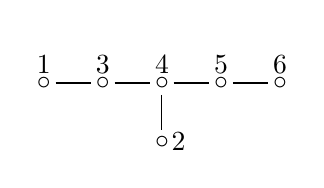
\begin{tikzpicture}[baseline = 20, scale=1.5]
\node at (-1,0) {$\circ$};
\node[above] at (-1, 0) {$1$};
\draw (-0.9,0) to (-0.6,0);
\node at (-0.5,0) {$\circ$};
\node[above] at (-0.5, 0) {$3$};
\draw (-0.4,0) to (-0.1,0);
\node at (0,0) {$\circ$};
\node[above] at (0, 0) {$4$};
\draw (0.1,0) to (0.4,0);
\node at (0.5,0) {$\circ$};
\node[above] at (0.5, 0) {$5$};
\draw (0.6,0) to (0.9,0);
\node at (1,0) {$\circ$};
\node[above] at (1, 0) {$6$};
\draw (0,-0.1) to (0,-0.4);
\node at (0,-0.5) {$\circ$};
\node[right] at (0, -0.5) {$2$};
\end{tikzpicture}
\] The $\d$-obits on $\Pi$ are $\{1, 6\}$, $\{3, 5\}$, $\{2\}$ and $\{4\}$. So $V(\d, \pi)$ is spanned by $(1, 0, 0, 0, 0, -1)$ and $(0, 0, 1, 0, -1, 0)$. Here $\mu=(\mu_1, \dots, \mu_6) \in \mathbb Z^6$ stands for the vector $\sum_{i=1}^6 \mu_i \a_i^\vee \in \mathbb Z \D^\vee$. One checks that the root system $\D' = \{\a \in \D; \langle \a, V(\d, \pi)\rangle=0\}$ is of type $D_4$, which is conjugate to the root system $\D''$ spanned by $\{2, 3, 4, 5\} \subseteq \Pi$. Up to $W$-conjugation, we can assume $\D_1 = \D''$.

Now one computes that $\l_1^\vee = \rho_1^\vee=(0, 3, 3, 5, 3, 0)$ and its dominant conjugate is $\overline{\l_1^\vee}=(3, 5, 6, 9, 6, 3)$. Note that $\rho^\vee=(8, 11, 15, 21, 15, 8)$. Then full sequence gives $$t=\d \exp(\frac{2\pi i}{6} \l_0) = \d \exp(\frac{2\pi i}{6} (\rho^\vee + \overline{\l_1^\vee}))=\d \exp(\frac{2\pi i}{6} (11, 16, 21, 30, 21, 11)).$$ The partial sequence gives $$t'= \d \exp(\frac{2\pi i}{3} \rho^\vee)=\d \exp(\frac{2\pi i}{6} (16, 22, 30, 42, 30, 16)).$$ So $t \neq t'$. On the other hand, we have \begin{gather*} t_1:=n_{s_1 s_6} t n_{s_1 s_6}^{-1} = \d \exp(\frac{2\pi i}{6}(10, 16, 21, 30, 21, 10)); \\ t_2:=\a_3^\vee(-1) t_1 \a_3^\vee(-1)=\d \exp(\frac{2\pi i}{6}(10, 16, 18, 30, 24, 10))=t'.\end{gather*} So $t$ is conjugate to $t'$.

\sec{The inductive step}

\subsection{The element $\l_0^\vee$ is $\d$-stable} Note that if the elements $w, w' \in {}^\d W$ are conjugate by an element of $W$, then the sequences $\{F_i\}, \{\D_i\}, \{W_i\}$ associated to $w$ and $w'$ are also conjugate under the action of $W$. Thus by replacing $w$ by a suitable element in its conjugacy class, we may assume that the dominant chamber $\caC$ is in good position with $w$. Let $w=\d x_1 x_2 \cdots x_k$ be the good factorization of $w$ as in Proposition \ref{good-fac}. We first show that the coweight $\l_0^\vee$ we constructed in section \ref{const} is fixed by $\d$.

\begin{lemma} \label{dom}
	We have $\l_0^\vee = \d(\l_0^\vee)$.
\end{lemma}
\begin{proof}
    Recall that $\d_i=\d x_1 \cdots x_{i}$. We show by induction that $\d_{i}(\l^\vee_{i})=\l^\vee_{i}$ for $0 \le i \le k$. If $i=k$, then $\l_k^\vee = 0$ and the statement is obvious. Assume $\d_{i+1}(\l_{i+1}^\vee) = \l_{i+1}^\vee$ for some $0 \le i \le k-1$. We prove $\d_i(\l_i^\vee)=\l_i^\vee$. Since $\d_{i}(\D_i^+)=\D_i^+$, we have $$\d_{i}(\rho_i^\vee)=\rho_i^\vee.$$ Let $y_i \in W_i$ such that $\overline{\l_{i+1}^\vee} = y_i(\l_{i+1}^\vee)$. Then $$\overline{\l_{i+1}^\vee}=y_i \d_{i+1} y_i^{-1} (\overline{\l_{i+1}^\vee}) =y_i \d_i x_i y_i^{-1} (\overline{\l_{i+1}^\vee}).$$ Note that $y_i \d_i x_i y_i^{-1} \in \d_i W_i$ and that $\overline{\l_{i+1}^\vee}$ is dominant for $\D_i^+$. Therefore, $\d_i$ fixes $\overline{\l_{i+1}^\vee}$ and hence also fixes $\l_i^\vee$ as desired.
\end{proof}

\subsection{The lifting $n(x)$}\label{setup}

We may regard $\d \circ \Ad(x_1)$ as an automorphism of $W_1$ and of the Levi subgroup $L_{\Pi_1}$ associated to $\Pi_1$. Then $\d_1 (x_2 \cdots x_k)$ is an elliptic element of $W_1 \rtimes \langle\d \circ \Ad(x_1)\rangle$. Thus by inductive hypothesis on the Levi subgroup associated to $\Pi_1$, we have that

(a) $n_w$ is conjugate to $n_{\d_1} \exp(\frac{2 \pi i \l^\vee_1}{d}) \in L_{\Pi_1} \rtimes \langle\d \circ \Ad(x_1)\rangle$.

In the next step, we would like to conjugate $n_{\d_1}$ to an element in $T \d$. Note that $\d_1$ is not an elliptic element of ${}^\d W$ in general.
Hence the lifting of $\d_1$ are not all conjugate in $G$. In particular, the Tits lifting of the elements in the conjugacy class of $\d_1$ are not all conjugate in $G$. For the purpose of our argument, we fix a set of lifts $n(x) \in N_G(T)$ for $x \in {}^\d W$ such that

(1) $n(s_\a)^2=\exp(\pi i \a^\vee)$ for $\a \in \Pi$;

(2) $n(x x') = n(x) n(x')$ if $\ell(x x') = \ell(x) + \ell(x')$.

We need a formula for the cycle defined by these lifts.

\begin{lemma} \label{factor}{\cite{ls}*{Lemma 2.1A}}
Given $x,y\in \Wext$ let 
$$
\gamma^\vee=\sum_{\g \in \D^+ \cap y \i(\D^-) \cap y \i x \i (\D^+)} \pi i \g^\vee).
$$
Then 
$$
n(x)n(y)=\exp(\pi i\gamma^\vee)n(xy)
$$
\end{lemma}


\begin{lemma} \label{average}
	Let $x \in W_0 \d$ and  $d \in \mathbb Z_{\ge 1}$ such that $x^d=1$. Let $\e \in V$. Then the element $n(x) \exp(2 \pi i \e)$ is conjugate to $n(x) \exp(\frac{2 \pi i}{d}\sum_{k=0}^{d-1} x^k(\e))$ by an element in $T$.
\end{lemma}
\begin{proof}
	Let $$r=\exp(\frac{2\pi i }{d}\sum_{k=0}^{d-1} k x^{-k}(\e)).$$ Then $r^{-1} n(x) \exp(2 \pi i \e) r = n(x) \exp(2\pi i\frac{1}{d}\sum_{i=0}^{d-1} x^i(\e))$ as desired.
\end{proof}

\subsection{Analysis of the element $n(\d_1)$}

We first show that

\begin{lemma}
	Let $\D'=\{\a \in \D; \langle\a, V^{\d_1}\rangle=0\}$ and let $V'$ be the subspace of $V$ spanned by $\D'$. Then $V(\d_1, \th_1)$ contains a generic element of $V'$ with respect to the root system $\D'$.
\end{lemma}
\begin{proof}
	Let $\a \in \D'$. We have to show that $\langle\a, V(\d_1, \th_1)\rangle \neq \{0\}$. Assume otherwise. Then $\a \in \D_1$ since $V(w, \th_1) \subseteq V(\d_1, \th_1)$. On the other hand, as $\d_1(\D_1^+) = \D_1^+$, we have $\rho_1^\vee \in V^{\d_1}$. So $\langle\a, \rho_1^\vee \rangle = 0$, which is impossible. The proof is finished.
\end{proof}

Although $\d_1$ is ``regular'' with respect to $V'$, $n(\d_1)$ is not conjugate to $\d \exp(i \th_1 {\rho'}^\vee)$, where ${\rho'}^\vee=\sum_{\a \in {\D'}^+} \a^\vee$. In order to determine the element in $T \d$ that is conjugate to $n(\d_1)$, we first conjugate $\d_1$ to an element in a standard parabolic subgroup of $W$.

By the algorithm and Lemma \ref{dom}, $\l_1^\vee$ is $\Pi_1$-dominant and is in $V^{\d_1}$. Set $\phi_1^\vee = \l_1^\vee + \frac{d \th_1}{2 \pi}\rho_1^\vee \in V^x$. Then $\phi_1^\vee$ is also $\Pi_1$-dominant and is in $V^{\d_1}$.

Let $v$ be a general point of $V^{\d_1}$ lying in a sufficiently small neighborhood of $\phi_1^\vee$. As $\phi_1^\vee \in V^{\d_1}$ is $\Pi_1$-dominant and that the (open) $\Pi_1$-dominant chamber intersects $V^{\d_1}$, we can assume further that $v$ is also strictly $\Pi_1$-dominant. Let $z \in W_0$ be the (unique) minimal element such that $z\i(v) = \bar v$, the unique dominant $W_0$-conjugate of $v$. By the choice of $v$, we have $z^{-1}(\l_1^\vee)=\overline{\l_1^\vee}$. Let $K=J_{\bar v}$ and $y = z^{-1} \d_1 z$. As $y(\bar v)=\bar v$, we have $\d(\bar v)=\bar v$. This means that $y \in W_K \d$ and $\d(K)=K$. Similarly, we have $\overline{\phi_1^\vee} = \d(\overline{\phi_1^\vee})$.

Notice that $\ell(z y)=\ell(z) + \ell(y)$. By Lemma \ref{factor} one has \begin{align*} n(\d_1) &= n(z y z^{-1}) \\ &= n(z y) n(z^{-1}) \exp(\sum_{\g \in \D^+ \cap z(\D^-) \cap \d_1 \i (\D^+)} -\pi i \g^\vee) \\ &= n(z) n(y) n(z^{-1}) \exp(\sum_{\g \in \D^+ \cap z(\D^-) \cap \d_1 \i (\D^+)} -\pi i \g^\vee) \\ &= n(z) n(y) n(z)^{-1} \exp(\sum_{\g \in \D^+ \cap z(\D^-) \cap \d_1 \i(\D^-)} \pi i \g^\vee), \end{align*} where the last equality follows from $$n(z^{-1})=n(z)^{-1} \exp(\sum_{\g \in \D^+ \cap z(\D^-)} \pi i \g^\vee).$$

\subsection{A technical lemma}

\begin{lemma} \label{tech}
	Let notation be as in above. We have $$\D^- - z \i(\D_{\Pi_1})-\D_K = \cup_{i=0}^{d-1} y^{-i}(\D^- \cap z \i(\D^+) \cap z \i \d_1 \i(\D^-)).$$ Moreover, each root of $\D^- - z \i(\D_{\Pi_1})-\D_K$ lies in exactly $\frac{d \th_1} {2\pi}$ of the sets $y^{-i}(\D^- \cap z \i(\D^+) \cap z \i \d_1 \i(\D^-))$ for $0 \le i \le d-1$.
	
%\begin{enumerate}\item The element $y \in W$ acts on $\D^- - z \i(\D_{\Pi_1})-\D_K^-$;\item Each orbit is of size $\frac{2 \pi}{\th_1}$\item The set $\D^- \cap z \i(\D^+) \cap z \i \d_1 \i(\D^-)$ is a principal domain for the action of $y^{\frac{d \th_1}{2 \pi}}$.\end{enumerate}
\end{lemma}
\begin{remark}
The proof uses a similar method of counting root hyperplanes as in \cite[Lemma 2.1]{he_nie_minimal_finite}.
\end{remark}

\begin{proof}
	%(1) Recall that $\d_1 \in {}^{\Pi_1} ({}^\d W)^{\Pi_1}$ with $\d_1(\Pi_1)=\Pi_1$, $y=z \i \d_1 z \in W_K \d$, $z \in W^K$ and $\d(K)=K$.Since $y \in W_K \d$ and $\d(K)=K$, we have $y (\D^--\D_K^-)=\D^--\D_K^-$. On the other hand $y z \i(\D_{\Pi_1})=z \i \d_1(\D_{\Pi_1})=z \i (\D_{\Pi_1})$. Part (1) is proved.(3) We first show that $$\D^- \cap z \i(\D^+) \cap z \i \d_1 \i(\D^-) \subset \D^--z \i(\D_{\Pi_1})-\D_K^-.$$Let $\g \in \D^- \cap z \i(\D^+) \cap z \i \d_1 \i(\D^-)$.If $\g \in \D_K^-$, then $z(\g) \in \D^-$ since $z \in W^K$. That is a contradiction.If $\g \in z \i(\D_{\Pi_1})$, then $z (\g) \in \D_{\Pi_1} \cap \D^+=\D_{\Pi_1}^+$ and thus $\d_1 z(\g) \in \D_{\Pi_1}^+$. That is a contradiction.
	
   Set $\mathcal B= \D^- \cap z \i(\D^+) \cap z \i \d_1 \i(\D^-)$. Then we have
	
	(a) $\mathcal B=\{\b \in \D^-, H_\b \text{ separates $z^{-1}(\caC)$ from $\caC$ and $y^{-1} z^{-1}(\caC)$}\}$, where $H_\b \subseteq V$ denotes the root hyperplane of $\b$.
	
	Recall that $v_0$ is a general point of $V(\d_1, \th_1)$. For $i \in \mathbb Z$, set $v_i'=y^{-i} z^{-1} (v_0)$. Then the points $v_i'$ for $i \in \mathbb Z$ are contained in the subspace $D$ spanned by $v_0'$ and $v_1'$. In particular $\dim D \le 2$.
	
	We first consider the case where $\dim D=1$. In this case, we have $\th_1 = \pi$ and hence $w=-1$. Then $\D_{\Pi_1} = \emptyset$, $\d_1 = w$, $\D_K = \D$ and $z=1$. One checks that $\D^- - z \i(\D_{\Pi_1})-\D_K = \emptyset = \mathcal B$. So the statement follows.
	
	Now we consider the case where $\dim D=2$. Let $S \subseteq D$ the circle containing $v_i'$ for $i \in \mathbb Z$. Note that $v_i'=v_j'$ if $(i-j)\th_1/(2\pi) \in \mathbb Z$.
	
	As $z \in W^K$, $\D_K \cap \mathcal B = \emptyset$. Since $y \in W_K \d =\d W_K$, we have $y^{-i}(\mathcal B) \subseteq \D^- - \D_K$. Let $\g \in y^{-i}(\mathcal B)$. By (a), $H_\g$ separates $y^{-i} z^{-1} \caC$ from $y^{-i-1} z^{-1} \caC$. This means $\g \notin z^{-1}(\D_{\Pi_1})$ as $x(\Pi_1)=\Pi_1$. So $y^{-i}(\mathcal B) \subseteq \D^- - z^{-1}(\D_{\Pi_1}) -\D_K$.
	
	Let $\b \in \D^- - z^{-1}(\D_{\Pi_1}) -\D_K$. If $v_k' \in H_\b$ for some $k$, then $z^{-1}(V_{\th_1}) \subseteq H_\b$ since $v_k'=y^{-k} z^{-1}(v_0)$ is a general point of $z^{-1}(V_{\th_1})$. This means $\b \in z^{-1}(\D_{\Pi_1})$, a contradiction. So $v_i' \notin H_\b$ for any $i \in \mathbb Z$. Thus, $H_\b \cap S = \{\pm p\}$ for some $p \in S$.
	
	Let $\overline\caC$ be the closure of $\caC$. Recall that $v$ is a general point of $V^{\d_1}$. As $\b \notin \D_K$ and $\bar v \in \overline\caC$, one deduces that
	
	(b) $\bar v \notin H_\b$ and that $y^{-i}(\bar v)=\bar v, y^{-i}(\caC)$ are on the same side of $H_\b$ for $i \in \mathbb Z$.
	
	Similarly, one has
	
	(c) $v_i', y^{-i} z^{-1}(\caC)$ are on the same side of $H_\b$ for $i \in \mathbb Z$.
	
	Let $S^+, S^-$ be the two connected components of $S - \{\pm p\}=S - H_\b$ such that $\bar v, S^+$ are on the same side of $H_\b$. In view of (a), (b) and (c), one has
	
	(d) $\b \in y^{-i}(\mathcal B)$ if and only if $v_i' \in S^-$ and $v_{i+1}' \in S^+$.
	
	Notice that the acute arc $(v_i', v_{i+1}')$ is of angle $0 < \th_1 < \pi$. It follows that that the number of integers $0 \le i \le d-1$ satisfying the condition (d) is exactly $d\th_1/2\pi$. The proof is finished.
\end{proof}

\begin{figure}
\center
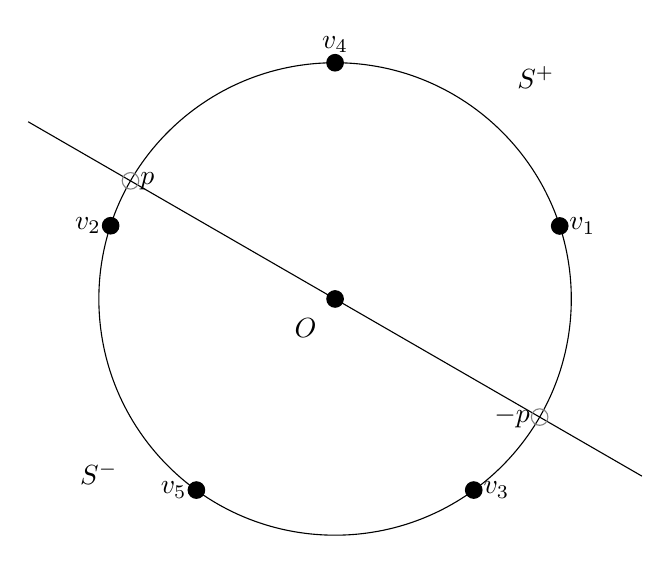
\begin{tikzpicture}[scale=1.5]


%\draw[step=1,color=gray!40] (-2,-2) grid (2,2);
 \draw[-] (-2.598,1.5) -- (2.598,-1.5) ;
  \path (1.7,1.7) node[above]{$S^{+}$};
  \path (-2,-1.3) node[below]{$S^{-}$};
 \draw (0,0) circle (2);
 \path (-0.25,-0.25) node(axis0){$O$};
 \draw[fill, black] (0,0) circle [radius=.07cm];
 \path (-1.732,1) node(text1)[right]{$p$};
 \draw[gray] (-1.732,1) circle [radius=.07cm];
\path (1.732,-1) node(text2)[left]{$-p$};
\draw[gray] (1.732,-1) circle [radius=.07cm];
\path (0,2) node(text3)[above]{$v_4$};
\draw[fill, black] (0,2) circle [radius=.07cm];
\path (1.902,0.618) node(text4)[right]{$v_1$};
 \draw[fill, black] (1.902,0.618) circle [radius=.07cm];
 \path (-1.9,0.62) node(text4)[left]{$v_2$};
 \draw[fill, black] (-1.9,0.62) circle [radius=.07cm];
 \path (1.174,-1.618) node(text4)[right]{$v_3$};
 \draw[fill, black] (1.174,-1.618) circle [radius=.07cm];
 \path (-1.174,-1.618) node(text4)[left]{$v_5$};
 \draw[fill, black] (-1.174,-1.618) circle [radius=.07cm];
\end{tikzpicture}

\caption{This is an illustration for the proof of Lemma \ref{tech}. Here $d=5$ and $\th_1 = \frac{4\pi}{5}$. The straight line is the intersection $H_\b \cap D$.}
\end{figure}

\begin{exampleplain}
	Let $W$ be of type $B_3$ and $\Pi=\{1, 2, 3\}$ such that $\a_3$ is the unique short simple root and $s_{13} = s_{31}$. Let $w=s_{12323}$. Then $\th_1 = \pi/2$, $d = 4$ and $w = \d_1 w_1$, where $\d_1 = s_{1232}$, $w_1 = s_3$, $\Pi_1=\{3\}$ and $V^{\d_1} = \mathbb R \a_3$. As in \ref{setup}, we take $v = \a_3$. Hence $z = s_{21}$, $y = s_{23}$ and $K=\{2, 3\}$. One checks that each root of $\D^- - z\i(\D_{\Pi_1}) - \D_K=\{-(\a_1), -(\a_1+\a_2), -(\a_1+\a_2+2 \a_3), -(\a_1+2 \a_2+2 \a_3)\}$ appears exactly one of the sets $\{-y^i(\a_1+\a_2)\}$ for $0 \le i \le 3$.
\end{exampleplain}

\subsection{Proof of Theorem \ref{t:main}}
\begin{comment}
\begin{proposition} \label{formula}
Let $e = d\th_1/2\pi$. Then $$n(w) \sim \d \exp(2\pi i\frac{e\rho^\vee + \overline{\l_1^\vee}}{d}).$$
\end{proposition}
Notice that $e\rho^\vee + \overline{\l_1^\vee}$ is dominant and is fixed by $\d$.

\begin{proof}
	Let $\mathcal B =z^{-1}((\D^+ \cap z(\D^-)) - \mathcal F(x z, z^{-1}))$ and $t=\exp (\pi i \sum_{\g \in \mathcal B} \g^\vee)$. Thanks to Lemma \ref{tech} below and that $y$ is elliptic for $\D_K$ we have $$\prod_{0 \le j \le d-1} y^j(t)=\exp(2\pi i e (\rho^\vee-z^{-1}(\rho_J^\vee)-\rho_K^\vee)).$$
\end{comment}
By inductive hypothesis, $n(w)$ is conjugate to $n(\d_1) \exp(\frac{2 \pi i \phi_1^\vee}{d})$ and hence conjugate to $n(z)^{-1} n(\d_1) \exp(\frac{2 \pi i \phi_1^\vee}{d}) n(z)$.

We have $$n(z)^{-1} n(\d_1) \exp(\frac{2 \pi i \phi_1^\vee}{d}) n(z)=n(y) t \exp(\frac{2 \pi i z^{-1}(\phi_1^\vee)}{d}),$$ where $t=\exp (\sum_{\g \in \D^+ \cap z(\D^-) \cap \d_1 \i(\D^-)} \pi i z^{-1}(\g^\vee))$. By Lemma \ref{tech}, $$\prod_{0 \le j \le d-1} y^j(t)=\exp(2\pi i e (\rho^\vee-z^{-1}(\rho_{\Pi_1}^\vee)-\rho_K^\vee)).$$

For any subgroup $H$ of $G$ and $g, g' \in {}^\d G$, we write $g \sim_H g'$ if $g'=h g h \i$ for some $h \in G$.

Let $L_K$ is the standard Levi subgroup of $G$ with root system $\D_K$. We have \begin{align*} n(w) &\sim_G  n(y) t \exp(\frac{2 \pi i z^{-1}(\phi_1^\vee)}{d}) \\ & \sim_T n(y) \exp(\frac{2\pi i e (\rho^\vee-z^{-1}(\rho_{\Pi_1}^\vee)-\rho_K^\vee)}{d}) \exp(\frac{2 \pi i z^{-1}(\phi_1^\vee)}{d}) \\ & \sim_{G_K} \d \exp(\frac{2 \pi i e \rho_K^\vee}{d}) \exp(\frac{2\pi i e (\rho^\vee-z^{-1}(\rho_{\Pi_1}^\vee)-\rho_K^\vee)}{d}) \exp(\frac{2 \pi i z^{-1}(\phi_1^\vee)}{d}) \\ &=\d \exp(\frac{2\pi i (e\rho^\vee + z^{-1}(\phi_1^\vee - e\rho_{\Pi_1}^\vee))}{d}) \\ &=\d \exp(\frac{2\pi i (e\rho^\vee + \overline{\l_1^\vee})}{d})=\d \exp(\frac{2 \pi i \l_0^\vee}{d}).
\end{align*} Here the second conjugation follows from Lemma \ref{average}; the third one follows from Proposition \ref{regular} and that $\rho^\vee-z^{-1}(\rho_{\Pi_1}^\vee)-\rho_K^\vee, z^{-1}(\phi_1^\vee)$ are central for $G_K$. The proof is finished.
%\end{proof}
\sec{Kac diagrams}

\sec{Table}

\bibliographystyle{plain} 
\bibliography{./refs.bib}

\end{document}
%%% Local Variables:
%%% mode: latex
%%% TeX-master: t
%%% End: s_{1}:0 -> -1 6









